\chapter{Experimental Results}
\label{ch:experiments}

\section{Experimental Design}
\label{sec:expiremental_design}

Following the completion of AFLuent, an evaluation step is needed to understand
how accurate the tool is in localizing faults. This section discusses the design
of this experiment including early steps in choosing and filtering a sample to
test AFLuent on.

\subsection{Approach Overview}
\label{subsec:approach_overview}

In order to evaluate AFLuent, several prerequisites are needed that enable
collecting data for analysis. The primary requirement is a collection of Python
program, which are susceptible of becoming faulty. Additionally, this
collection's complexity must be comparable to code typically written by novice
developers, which AFLuent targets. Another crucial requirement before evaluation
can begin is a test suite for the selected code python code. The test suite must
be executable by Pytest and covers as much as possible of the code under test to
maximize the ability to localize faults. Assuming that these prerequisites are
met and are available, the evaluation of AFLuent can then be generally described
by these four main steps:

\begin{enumerate}
    \item Introduce a bug/fault in the code under test
    \item Run the test suite with AFLuent
    \item Produce a report of suspicious statements as ranked by AFLuent
    \item Asses how far the in the produced ranking report was the location of
    the introduced bug
\end{enumerate}

While these steps are great for planning and describing the intention in evaluating
AFLuent, they fall short of providing a clear and detailed plan. The sections
below will expand on the points discussed here and elaborate on how the
prerequisites are met and describe the systematic and automated approach in evaluation.

\subsection{Research Questions}
\label{subsec:research_questions_eval}

Before discussing the evaluation process, it's important to clearly state the
questions to answer. Previously, Section\ref{sec:researchq} brought up few
research question concerning the implementation and evaluation of AFL in Python.
Related Work and Methods section addressed \emph{RQ1.1} as well as
\emph{RQ2}, however, the answer \emph{RQ1.2} remains unclear. While \emph{RQ1.2}
generally involved the efficiency and accuracy of AFLuent, there was no mention
of the metrics or the comparisons needed to achieve an answer. In general, there
are sixteen different approaches that will be evaluated and compared. For every AFL
equation used, Tarantula, Ochiai, Ochiai2, and Dstar, there are four tiebreaking
approaches. Each equation-tieberaker pair will be evaluated on the same dataset,
where the resulting rankings will be used to produce a score to assess how
close the produced ranking are to localizing the fault correctly. In addition to
this score, the time taken to run each approach will be recorded to compare
their time overhead.

\subsection{Choosing a Sample}
\label{subsec:choosing_sample}

Since AFLuent is targeted towards novice developers with little experience
programming in Python, the evaluation strategy should reflect that by running
AFLuent on novice written code. However, considering that this study does not
involve human subjects, novice developers cannot be asked to write code for the
purposes of this evaluation. To simulate novice written code as best as
possible, the GitHub repository \code{TheAlgorithms/Python}\cite{the_algorithms_python}
is used as the sample. This educational repository is a collection of projects
that implement several fundamental algorithms in Python that range from ciphers,
sorting, graphs, string operations to financial and physics equations.
It resembles novice written
code because, in a sense, beginner developers write these programs while
learning the basics of programming. However, a problem
with using this code is the lack of unit tests that pytest can run, since most
tests are written using Python's doctest. With that in mind, there are Python
tools such as Pynguin\cite{Lukasczyk_Pynguin_Automated_Unit_2022}
that can be used to automatically generate a test suite for these projects.
With the many limitations in Pynguin and the long waiting times to generate
tests, some filtering of the projects is needed.


\subsubsection{Filtering Sample}
\label{subsubsec:filtering_sample}

There are many issues that could arise when automatically generating a test
suite using Pynguin. To mitigate these problems, the following criteria was used
to eliminate entire projects, delete modules, or trim some code.

\begin{itemize}
    \item Projects that import external modules: In order to facilitate and
    expedite generating a test suite using Pynguin, several projects that use
    external packages were removed. These packages include \code{scikit-learn},
    \code{Tensorflow}, \code{Matplotlib}, \code{Sympy}, and \code{PIL}.
    Generating data and creating unit tests for projects that using theses
    packages can be difficult because they are time consuming or simply cannot
    be tested due to their graphical output.
    \item Functions that do not take input or return no results: some implemented
    functions do not accept arguments as input. This makes them difficult to
    test because no data can be passed to them. Additionally, functions that do
    not return a result are also difficult because there is no output to be
    checked. Functions that are part of an object oriented structure that change
    the state of an object without returning a value were kept since their
    results can be tested. However, other functions such as \code{main()} which
    read input from the console and controlled the flow were removed.
    \item Functions with missing type hints in signature: generating data for
    functions with unknown input type would be challenging for Pynguin to
    perform. Therefore, these functions were removed. In some instances where
    the documentation explicitly stated the type of input for the function, type
    hints were manually added to avoid the removal of the function. This was
    especially frequent in sorting function, in which the input was specified as
    integer values.
    \item Code snippets under \code{if \_\_name\_\_ == "\_\_main\_\_"}: In most
    instances the code under this if statement either ran the doctest tests, or
    called a separately implemented main function. Since there is no use for
    these snippets and to clean up the sample, these snippets were removed.
\end{itemize}


\begin{table}[!htb]
    \centering
	\begin{tabular}{|c|c|c|c|}
        \hline
        arithmetic\_analysis & audio\_filters   & backtracking       & bit\_manipulation    \\
        blockchain           & boolean\_algebra & cellular\_automata & ciphers              \\
        compression          & conversions      & data\_structures   & divide\_and\_conquer \\
        dynamic\_programming & electronics      & financial          & genetic\_algorithm   \\
        geodesy              & graphs           & greedy\_methods    & hashes               \\
        knapsack             & linear\_algebra  & maths              & matrix               \\
        physics              & scheduling       & searches           & sorts                \\
        strings              &                  &                    &\\

        \hline
	\end{tabular}
	\caption{Remaining Projects Prior to Test Generation}
	\label{table:remaining_projects}
\end{table}

Following the initial phase of filtering the codebase, general statistics and
observations were recorded for the remaining sample thus far.
Table\ref{table:remaining_projects} shows the name of the remaining project.
Additionally, SLOCcount was used to calculate the number of non-comment line of
code included in the sample. The output from the tool is shown in
Fig\ref{fig:SLOCcount_phase1}. Overall, there was 12199 lines of code remaining
in the sample prior to automatically generating tests using Pynguin.

\begin{figure}[!htb]
	\begin{center}
		\begin{lstlisting}
            SLOC	Directory	SLOC-by-Language (Sorted)
            2396    data_structures python=2396
            1856    ciphers         python=1856
            1583    maths           python=1583
            900     graphs          python=900
            664     sorts           python=664
            559     strings         python=559
            543     conversions     python=543
            412     linear_algebra  python=412
            365     divide_and_conquer python=365
            360     matrix          python=360
            359     dynamic_programming python=359
            308     backtracking    python=308
            248     compression     python=248
            236     searches        python=236
            200     arithmetic_analysis python=200
            173     hashes          python=173
            171     audio_filters   python=171
            161     bit_manipulation python=161
            118     cellular_automata python=118
            109     boolean_algebra python=109
            97      scheduling      python=97
            94      blockchain      python=94
            86      electronics     python=86
            67      genetic_algorithm python=67
            43      financial       python=43
            40      knapsack        python=40
            37      geodesy         python=37
            11      greedy_methods  python=11
            3       physics         python=3

            Totals grouped by language (dominant language first):
            python:       12199 (100.00%)
        \end{lstlisting}
		\caption{\label{fig:SLOCcount_phase1} SLOCcount Output After Initial Filtering}
	\end{center}
\end{figure}


\subsubsection{Generating a Test Suite}
\label{subsubsec:generating_test_suite}

Once initial filtering of the codebase was completed, Pynguin was ran to
generate tests. However, additional issues came up in this process that required
additional filtering to be done. The new content was filtered as follows:
\begin{itemize}
    \item When attempting to generate tests,
    Pynguin failed in 54 modules and threw error messages indicating possible
    bugs in the tool. To limit the time taken to generate tests, 15 minutes were
    given per module, where no tests were generated for 73 modules due to
    getting timed out. Finally, there were 249 modules where tests were
    successfully generated. Modules with failed and timed out runs were removed
    due to the lack of tests that cover them.
    \item Some generated tests were faulty and caused errors when ran, or
    indeterminately failed making them flaky. Those tests were removed in some
    instances or fixed when possible.
    \item Since AFLuent relies on a thorough test suite with high coverage in
    order to find bugs accurately, modules with below 85\% coverage were removed.
\end{itemize}

\begin{figure}[!htb]
	\begin{center}
		\begin{lstlisting}
            SLOC	Directory	SLOC-by-Language (Sorted)
            934     maths           python=934
            826     ciphers         python=826
            576     data_structures python=576
            496     sorts           python=496
            465     conversions     python=465
            454     graphs          python=454
            356     strings         python=356
            217     dynamic_programming python=217
            192     backtracking    python=192
            173     hashes          python=173
            133     bit_manipulation python=133
            101     searches        python=101
            90      linear_algebra  python=90
            69      electronics     python=69
            61      divide_and_conquer python=61
            43      financial       python=43
            42      scheduling      python=42
            37      geodesy         python=37
            27      knapsack        python=27
            16      arithmetic_analysis python=16
            14      cellular_automata python=14
            11      greedy_methods  python=11
            10      compression     python=10
            3       physics         python=3

            Totals grouped by language (dominant language first):
            python:        5346 (100.00%)

        \end{lstlisting}
		\caption{\label{fig:SLOCcount_phase2} SLOCcount Output After Initial Filtering}
	\end{center}
\end{figure}

\begin{figure}[!htb]
	\begin{center}
		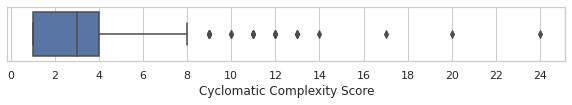
\includegraphics[width=15.5cm]{cyclomatic_complexity.png}
		\caption{\label{fig:cyclomatic_complexity_of_sample} Cyclomatic
		Complextiy of Sample}
	\end{center}
\end{figure}

After the second filtering step SLOCcount statistics were collected again to get
information on the sample, the output from the tool is shown in
Fig.\ref{fig:SLOCcount_phase2}. While the codebase was significantly reduced in
size, the resulting test suite contains 1105 test cases with 99\% coverage.
In order to get a better understanding of the remaining sample, additional data
was collected on the cyclomatic complexity the functions in the code. This
information would give some ideas on the structure of the code regarding if
statements, loops and other constructs. The cyclomatic complexity of the
remaining 516 functions was calculated and plotted as shown on
\ref{fig:cyclomatic_complexity_of_sample}. The plot shows a median cyclomatic
complexity of 3 for most functions with few outliers ranging to 24. While these
results mean that the code is very linear, they also suggest that it resembles
what novice developers write.

\section{Evaluation}

\emph{TODO: add information}

% !Single mutation evaluation

\section{Threats to Validity}